\documentclass[12pt]{report}
\usepackage[utf8]{inputenc}
\usepackage{graphicx}
\usepackage{amsmath}
\usepackage{hyperref}
\usepackage{makecell}
\usepackage{adjustbox}
\usepackage{geometry} 
\usepackage{subcaption}
\usepackage{float}

\title{Assignment 4: \\ Optimization with Genetic Algorithms \\ Neuronal and evolutionary computing\\ 2023 - 2024}
\author{Pawel Puzdrowski}
\date{2024-01-13}

\begin{document}
    \maketitle
    \tableofcontents
    \newpage
    \section{Git repository}
    The repository that holds the code for this assignment can be found on this website: https://github.com/Pawel712/NEC-Assignment4.git
    \section{Description of the chromosome, and adaptations done to the algorithm}
    \subsection{Translation of the problem to chromosome}
    Firstly the dataset is imported with help of tsplib95 library. A simple tsplib95.load() function is used to import the dataset and get proper structure of the problem so it can be handled by the genetic algorithm. The genetic algorithm has several stages and this stages are inspired from geeksforgeeks source \cite{TSPGeeksforgeeks}
    \begin{itemize}
        \item Initialization 
        \item Fitness score calculation
        \item Elitism 
        \item Selection 
        \item Crossover 
        \item Mutation 
        \item Population update 
    \end{itemize}
    At the initialization stage the original population is created with create$\_$initial$\_$population() function. The cities are extracted from the dataset and tours are created randomly. \\
    \\
    Fitness score calculation is done with fitness() function where following fitness score calculation is done:\\
    \\
    $\frac{1}{calculate_distance()}$\\
    \\
    Function calculate$\_$distance() is basically calculating the total distance of a tour. Then if the distance is high the fitness score will get low and if the distance is low the fitness score will get high. Every tour is assigned one fitness score. \\
    \\
    The part where elitism is done, it's taken from this source \cite{Elitismsource}. Elitism is done with elitism() function. The best tour from the population is chosen and added to the new population. This way the best tour is always saved in the new population and the evolution is faster.\\
    \\
    Selection is choosing the parents for the mating part. Depending on the method the parents are choosen differently. Crossover section is creating the children from the chosen parents and depedning on the method the childrens inheritance of parents genetics is done. Mutation part has the responsibility to perform mutations on the children and as well mutation has different methods to perform mutations so the mutations can vary.\\
    \\
    To finish off the algorithm, all the parents creates a new child and at the end a new population has arrised and its selected to do the same mating process again depending on how many generations are specified.\\
    \\
    The different selection methods were taken from this source \cite{Elitismsource} and the different selection methods are listed below 
    \subsection{Methods for selection/crossover/mutation}
    Selection methods: \cite{Elitismsource}
    \begin{itemize}
        \item Fitness proportionate selection (selectionFPS) - parents are choosen randomly, but the parents with higher fitness score has higher chance of being selected
        \item Tournament selection (selectionTS) - 4 parents are choosen randomly from the set and the parent with highest fitness score and the second highest score is chosen to mate.
    \end{itemize}
    Crossover methods: \cite{CrossoverSource} 
    \begin{itemize}
        \item One point crossover - a randomly point is chosen on the tour and the tour is splitted in two parts. Visualization of one point crossover is shown in figure \ref{fig:OnePointCross}
        \item Uniform crossover - each gene (city) is treated seperately instead of divided the parent in to one or more parts. Basically a flip-coin is done on every city if its included or not. Visualization of uniform crossover is shown in figure \ref{fig:uniformCrossover}
    \end{itemize}
    
    \begin{figure}
        \centering
        \includegraphics[scale=0.7]{images/onePointCross.png}
        \caption{One point cross}
        \label{fig:OnePointCross}
    \end{figure}

    \begin{figure}
        \centering
        \includegraphics[scale=0.7]{images/uniformCross.png}
        \caption{Uniform crossover}
        \label{fig:uniformCrossover}
    \end{figure}
    \noindent Mutation methods: \cite{MutationSource}
    \begin{itemize}
        \item One bit flip mutation - only one bit is mutated which in this case means that one city is swapped with another random city from the same tour. Visualization of one bit mutation is shown in figure \ref{fig:OneBitMutation}
        \item Scramble mutation - a random set of cities is chosen and swapped with another random set of cities. Visualization of scramble mutation is shown in figure \ref{fig:ScrambleMutation}
    \end{itemize}

    \begin{figure}
        \centering
        \includegraphics[scale=0.7]{images/oneBitMutation.png}
        \caption{One bit mutation}
        \label{fig:OneBitMutation}
    \end{figure}
    
    \begin{figure}
        \centering
        \includegraphics[scale=0.7]{images/ScrambleMutation.png}
        \caption{Scramble mutation}
        \label{fig:ScrambleMutation}
    \end{figure}
    
    \subsection{How the population size is chosen}
    After doing coople of test with population size, the best and efficient results are obtained when the population size of the size of the dataset or little bit higher. Double, tripple or higher population size doesn't result in better path.

    \subsection{How stationary state is identified}
    To identify stationary state for the datasets various tests were performed on the parameters: population size, number of generations, and mutation rate, and then checking the plot of evolution of the minimum total traveling distance. 

    \section{The results of executing the code for 5 problems of different sizes}

    \subsection{Description of the datasets}
    \textbf{smalldataset.tsp}\\
    Dataset consisting of only seven cities. This dataset is a modified att48.tsp where couple of points from the bigger dataset were taken and then added to the smaller dataset. This was done because there were no dataset to download that had less than 10 cities.\\
    \\
    \textbf{burma14.tsp}\\
    This dataset consist of 14 cities and was taken from this source \cite{DatasetSource}.\\
    \\
    \textbf{att48.tsp}\\
    This dataset consists of 48 cities and was taken from this source \cite{att48Data}.\\
    \\
    \textbf{ch150.tsp}\\
    Bigger dataset consisting of 150 cities and was taken from this source \cite{DatasetSource}.\\
    \\
    \textbf{a280.tsp}\\
    The biggest dataset consisting of 280 cities and was taken from this source \cite{DatasetSource}. Executing the program with bigger cities than that results in very long execution time. 
    \newpage
    \subsection{The results obtained with at least 6 different combinations of parameters}
    \textbf{smalldataset.tsp}\\
    \\
    The result from trying out different parameters for smalldataset is shown in table \ref{resultsSmallDataset}. The best results and evolution of best tour are shown in figures \ref{PlotsSmallDataset}. Because this is a very small dataset, it doesn't need much adjusting parameters to reach the best tour.
    \begin{table}
        \centering
        \begin{tabular}{|c|c|c|c|c|c|c|}
            \hline
            Pop size & Gen & Mutation & Selection & Cross & Mutation & Min Dist\\
            \hline
            20 & 100 & 0.1 & selectionFPS & OnePointcrossover & BitFlipMutation & 116 \\
            \hline
            40 & 100 & 0.2 & selectionFPS & OnePointcrossover & BitFlipMutation & 116 \\
            \hline
            40 & 10 & 0.1 & selectionFPS & OnePointcrossover & BitFlipMutation & 116 \\
            \hline
            40 & 100 & 0.2 & selectionTS & uniformCrossover & scramblemMutation & 116 \\
            \hline
            \end{tabular}
        \caption{Result dataset smallDataset.tsp}
        \label{resultsSmallDataset}
    \end{table}
    
	\begin{figure}[H]
		\centering
		\begin{subfigure}{.5\textwidth}
			\centering
			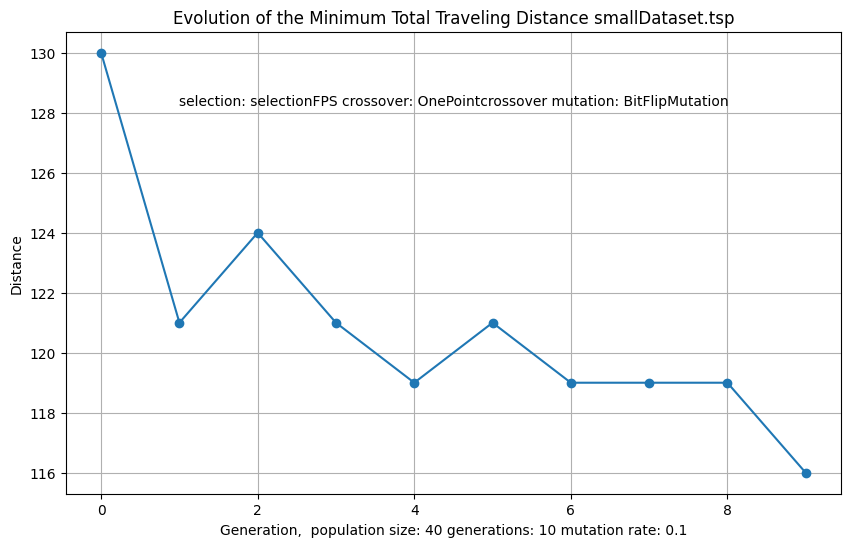
\includegraphics[width=.99\linewidth]{../Results/smallDataset/EvolutionPlot.png}
			\caption{Evolution of best tour}
			\label{EvolutionSmallDataset}
		\end{subfigure}%
		\begin{subfigure}{.5\textwidth}
			\centering
			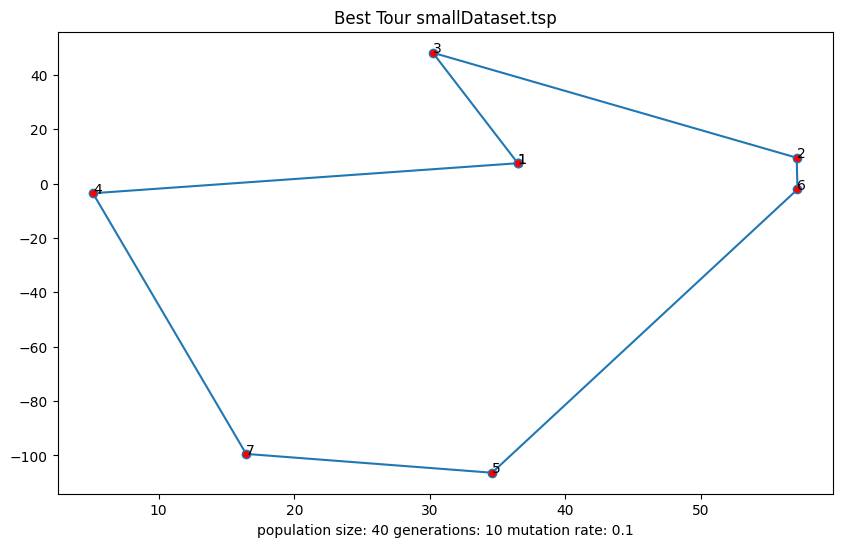
\includegraphics[width=.8\linewidth]{../Results/smallDataset/bestTour.png}
			\caption{Best tour}
			\label{bestTourSmallDataset}
		\end{subfigure}
		\caption{Plots for small dataset}
		\label{PlotsSmallDataset}
	\end{figure}
    \newpage
    \noindent \textbf{burma14.tsp}\\
    \\
    The result from trying out different parameters for burma14.tsp is shown in table \ref{resultsBurma14}. The best results and evolution of best tour are shown in figures \ref{Plotsburma14}. 
    \begin{table}
        \centering
        \begin{tabular}{|c|c|c|c|c|c|c|}
            \hline
            Pop size & Gen & Mutation & Selection & Cross & Mutation & Min Dist\\
            \hline
            40 & 10 & 0.1 & selectionFPS & OnePointcrossover & BitFlipMutation & 4814 \\
            \hline
            40 & 100 & 0.1 & selectionFPS & OnePointcrossover & BitFlipMutation & 4149 \\
            \hline
            40 & 100 & 0.2 & selectionFPS & OnePointcrossover & BitFlipMutation & 3642 \\
            \hline
            60 & 100 & 0.2 & selectionFPS & OnePointcrossover & BitFlipMutation & 3513 \\
            \hline
            60 & 200 & 0.2 & selectionFPS & OnePointcrossover & BitFlipMutation & 3346 \\
            \hline
            60 & 300 & 0.2 & selectionFPS & OnePointcrossover & BitFlipMutation & 3416 \\
            \hline
            60 & 200 & 0.2 & selectionTS & uniformCrossover & scramblemMutation & 3346 \\
            \hline
            \end{tabular}
        \caption{Result dataset burma14.tsp}
        \label{resultsBurma14}
    \end{table}

	\begin{figure}[H]
		\centering
		\begin{subfigure}{.5\textwidth}
			\centering
			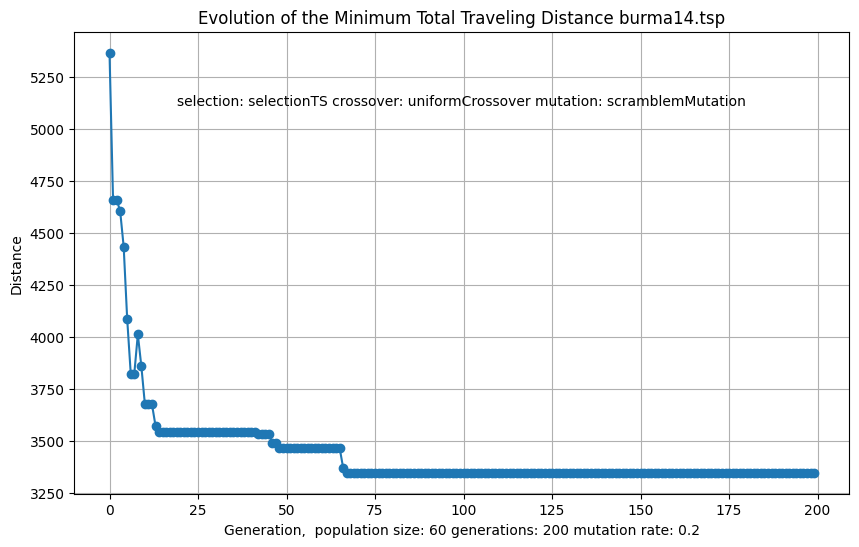
\includegraphics[width=.99\linewidth]{../Results/burma14/Evolution.png}
			\caption{Evolution of best tour}
			\label{Evolutionburma14}
		\end{subfigure}%
		\begin{subfigure}{.5\textwidth}
			\centering
			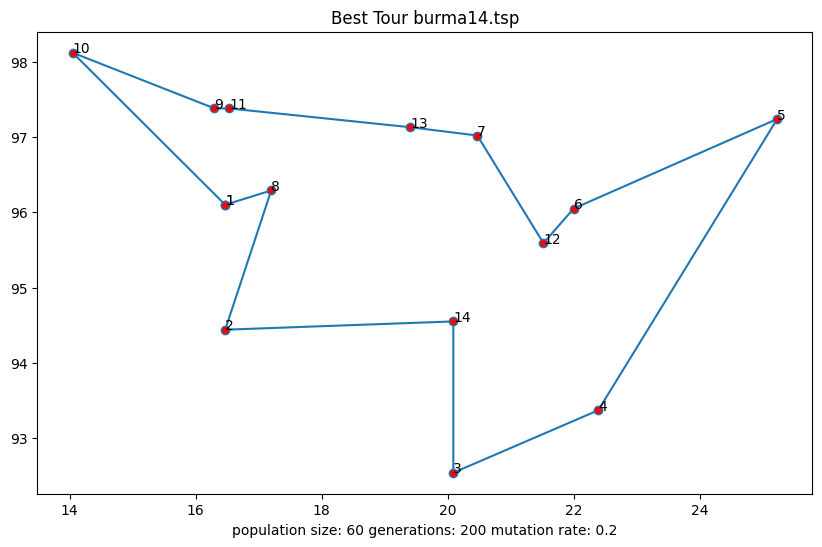
\includegraphics[width=.8\linewidth]{../Results/burma14/bestTour.png}
			\caption{Best tour}
			\label{bestTourburma14}
		\end{subfigure}
		\caption{Plots for burma14.tsp}
		\label{Plotsburma14}
	\end{figure}
    \newpage
    \noindent \textbf{att48.tsp}\\
    \\
    The result from trying out different parameters for att48.tsp is shown in table \ref{resultsatt48}. The best results and evolution of best tour are shown in figures \ref{Plotsatt48}.
    \begin{table}
        \centering
        \begin{tabular}{|c|c|c|c|c|c|c|}
            \hline
            Pop size & Gen & Mutation & Selection & Cross & Mutation & Min Dist\\
            \hline
            60 & 100 & 0.2 & selectionFPS & OnePointcrossover & BitFlipMutation & 31623 \\
            \hline
            100 & 100 & 0.2 & selectionFPS & OnePointcrossover & BitFlipMutation & 32467 \\
            \hline
            100 & 200 & 0.2 & selectionFPS & OnePointcrossover & BitFlipMutation & 29300\\
            \hline
            100 & 300 & 0.1 & selectionFPS & OnePointcrossover & BitFlipMutation & 25441 \\
            \hline
            100 & 200 & 0.1 & selectionTS & uniformCrossover & scramblemMutation & 21004 \\
            \hline
            150 & 200 & 0.1 & selectionTS & uniformCrossover & scramblemMutation & 19408 \\
            \hline
            \end{tabular}
        \caption{Result dataset att48.tsp}
        \label{resultsatt48}
    \end{table}

    \begin{figure}[H]
		\centering
		\begin{subfigure}{.5\textwidth}
			\centering
			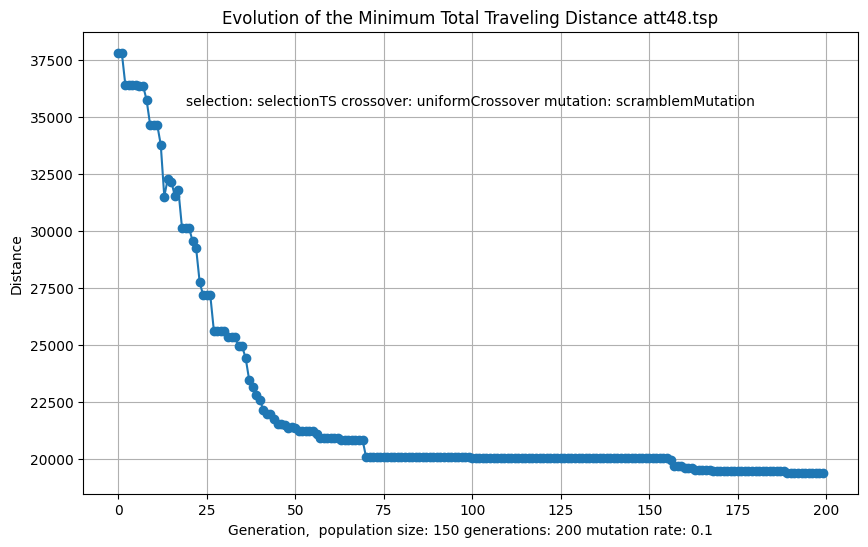
\includegraphics[width=.99\linewidth]{../Results/att48/Evolution.png}
			\caption{Evolution of best tour}
			\label{Evolutionatt48}
		\end{subfigure}%
		\begin{subfigure}{.5\textwidth}
			\centering
			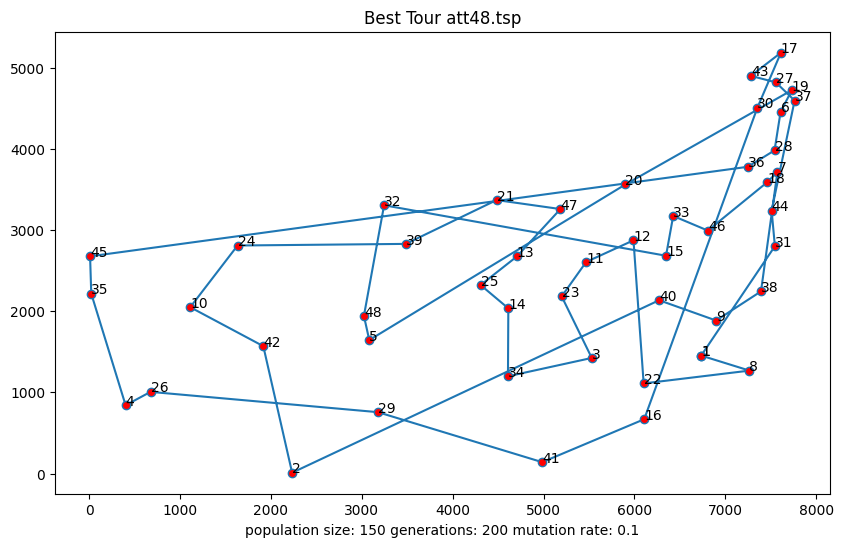
\includegraphics[width=.8\linewidth]{../Results/att48/bestTour.png}
			\caption{Best tour}
			\label{bestTouratt48}
		\end{subfigure}
		\caption{Plots for att48.tsp}
		\label{Plotsatt48}
	\end{figure}
    \newpage
    \noindent \textbf{ch150.tsp}\\
    \\
    The result from trying out different parameters for ch150.tsp is shown in table \ref{resultsch150}. The best results and evolution of best tour are shown in figures \ref{Plotsch150}.
    \begin{table}
        \centering
        \begin{tabular}{|c|c|c|c|c|c|c|}
            \hline
            Pop size & Gen & Mutation & Selection & Cross & Mutation & Min Dist\\
            \hline
            200 & 100 & 0.2 & selectionFPS & OnePointcrossover & BitFlipMutation & 45815 \\
            \hline
            200 & 100 & 0.1 & selectionFPS & OnePointcrossover & BitFlipMutation & 47187 \\
            \hline
            200 & 150 & 0.2 & selectionFPS & OnePointcrossover & BitFlipMutation & 45323 \\
            \hline
            200 & 150 & 0.2 & selectionTS & uniformCrossover & scramblemMutation & 25049 \\
            \hline
            200 & 300 & 0.2 & selectionTS & uniformCrossover & scramblemMutation & 19321\\
            \hline
            \end{tabular}
        \caption{Result dataset ch150.tsp}
        \label{resultsch150}
    \end{table}
    \begin{figure}[H]
		\centering
		\begin{subfigure}{.5\textwidth}
			\centering
			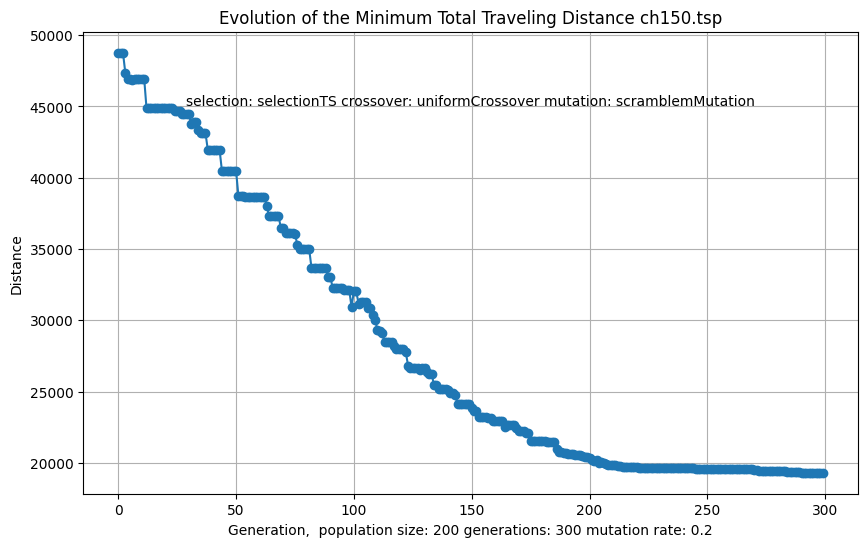
\includegraphics[width=.99\linewidth]{../Results/ch150/Evolution.png}
			\caption{Evolution of best tour}
			\label{Evolutionch150}
		\end{subfigure}%
		\begin{subfigure}{.5\textwidth}
			\centering
			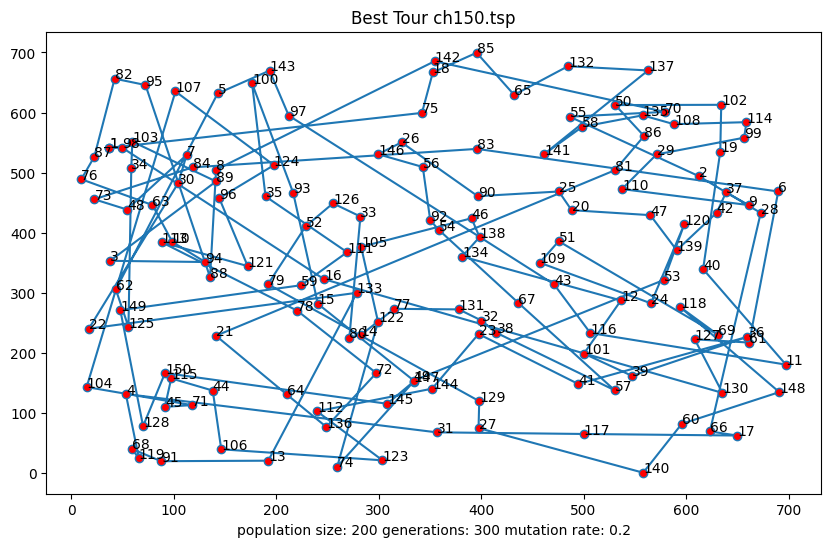
\includegraphics[width=.8\linewidth]{../Results/ch150/bestTour.png}
			\caption{Best tour}
			\label{bestTourch150}
		\end{subfigure}
		\caption{Plots for ch150.tsp}
		\label{Plotsch150}
	\end{figure}
    \newpage
    \noindent \textbf{a280.tsp}\\
    \\
    The result from trying out different parameters for a280.tsp is shown in table \ref{resultsa280}. The best results and evolution of best tour are shown in figures \ref{Plotsa280}.
    \begin{table}
        \centering
        \begin{tabular}{|c|c|c|c|c|c|c|}
            \hline
            Pop size & Gen & Mutation & Selection & Cross & Mutation & Min Dist\\
            \hline
            300 & 100 & 0.2 & selectionFPS & OnePointcrossover & BitFlipMutation & 29223 \\
            \hline
            300 & 100 & 0.1 & selectionFPS & OnePointcrossover & BitFlipMutation & 30058 \\
            \hline
            300 & 150 & 0.2 & selectionFPS & OnePointcrossover & BitFlipMutation & 28584 \\
            \hline
            300 & 150 & 0.2 & selectionTS & uniformCrossover & scramblemMutation & 20839 \\
            \hline
            300 & 250 & 0.2 & selectionTS & uniformCrossover & scramblemMutation & 15619 \\
            \hline
            \end{tabular}
        \caption{Result dataset a280.tsp}
        \label{resultsa280}
    \end{table}
    \begin{figure}[H]
		\centering
		\begin{subfigure}{.5\textwidth}
			\centering
			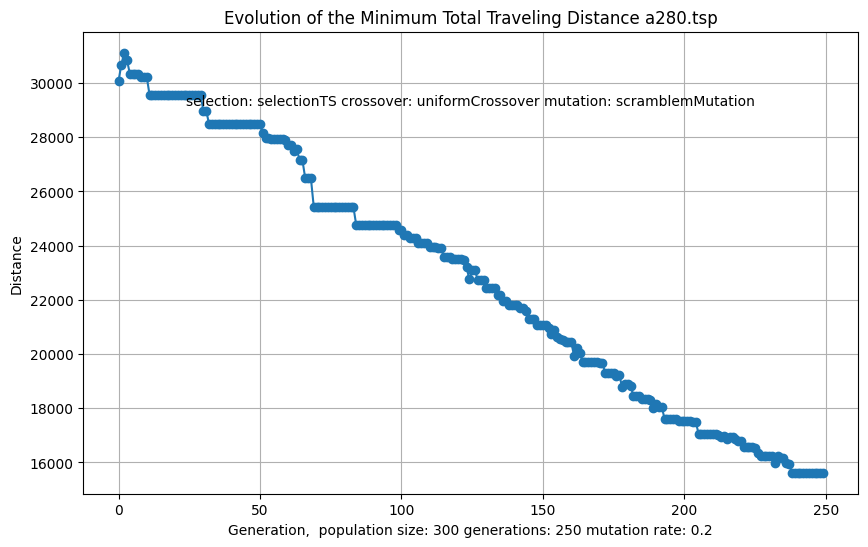
\includegraphics[width=.99\linewidth]{../Results/a280/Evolution.png}
			\caption{Evolution of best tour}
			\label{Evolutiona280}
		\end{subfigure}%
		\begin{subfigure}{.5\textwidth}
			\centering
			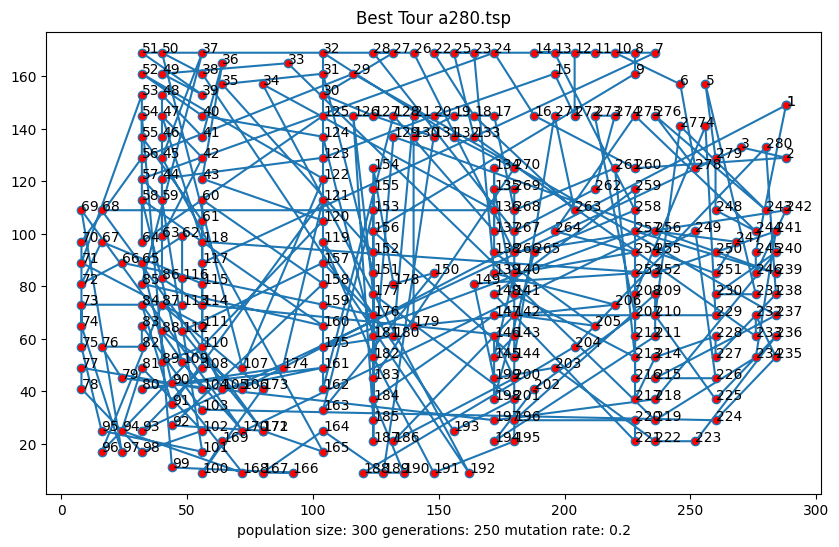
\includegraphics[width=.8\linewidth]{../Results/a280/bestTour.png}
			\caption{Best tour}
			\label{bestToura280}
		\end{subfigure}
		\caption{Plots for a280.tsp}
		\label{Plotsa280}
	\end{figure}
    \bibliographystyle{plainurl} 
	\bibliography{ref} 

    % Nästa gång:
    % göra tester på datasets och dokumentera det.

    %% Remember to include the git repo in the report. 
    %%  Look into what lambda does in the code


\end{document}